%
% Florent JACQUET - Romain THIBAUD - Antonin WALTZ
%
% Rapport de IN55 (P16)
%   Animation d'un personnage 3D avec OpenGL
%
%

\documentclass[a4paper]{report}
%packages
\usepackage[utf8]{inputenc}
\usepackage[francais]{babel}
\usepackage{graphicx}\graphicspath{{img/}}
\usepackage{float}
\usepackage[T1]{fontenc}
\usepackage{color}
\usepackage{fancyhdr}
\usepackage{listings}
\usepackage[colorlinks=true,allcolors=black]{hyperref}
\usepackage[font=small,labelfont=bf,margin=\parindent,tableposition=top]{caption}
\setcounter{tocdepth}{2}

\begin{document}
\begin{titlepage}
    
\includegraphics[width=0.4\textwidth]{logo_utbm.png}
    \begin{center}
        \textsc{\LARGE Université de Technologie de Belfort Montbéliard}\\[1cm]
        \textsc{\Large IN55}\\
        \rule{\linewidth}{0.5mm}
        { \huge \bfseries Animation d'un personnage 3D avec OpenGL\\[0.4cm] }
        \rule{\linewidth}{0.5mm}
        \vskip1cm
        % Author and supervisor
        Florent \textsc{Jacquet}\\
	Romain \textsc{Thibaud}\\
        Antonin \textsc{Waltz}\\
        Superviseur: Fabrice \textsc{Lauri}\\
        \vskip1cm
        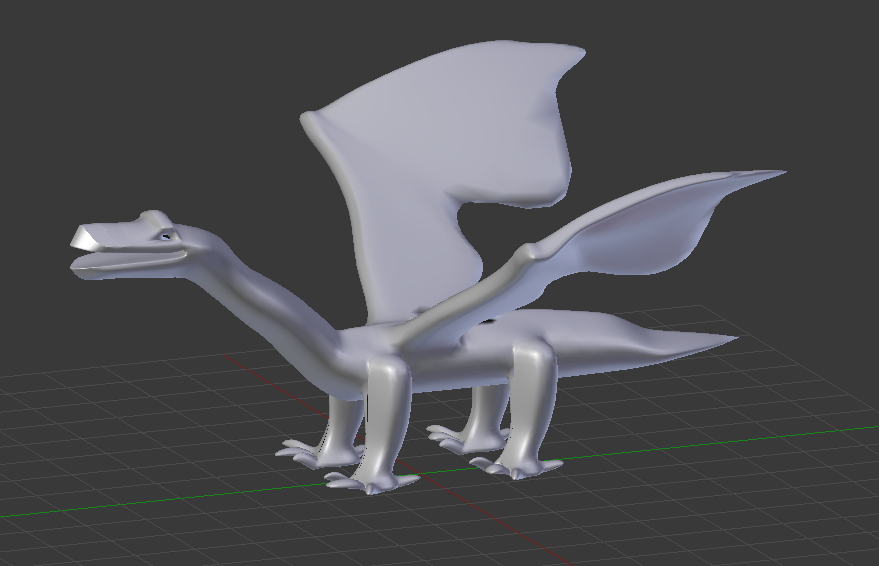
\includegraphics[width=0.6\textwidth]{dragon_front_page.png}
        \vfill
        {\large Printemps 2016}
    \end{center}
\end{titlepage}

\newpage
\tableofcontents
\listoffigures
\newpage
%%%%%%%%%%%%%%%%%%%%%%%%%%%%%%%%%%%%%%%%%%%%%%%%%%%%%%%%%%%%%%%%%%%%%%%%%%%%%%%%%%%%%%%%%%%%%%%%%%%%%%%
\chapter{Présentation du projet}
\par
Durant ce semestre en IN55, nous avons choisi le projet \textit{Animation d'un personnage 3D} parmi tout ceux proposés. Le personnage que nous avons modéliser et animer est un dragon. En effet, effectuer un rendu naturel de plusieurs mouvements (voler, marcher, s'asseoir) nous a sembler être un challenge intéressant.

\newpage
%%%%%%%%%%%%%%%%%%%%%%%%%%%%%%%%%%%%%%%%%%%%%%%%%%%%%%%%%%%%%%%%%%%%%%%%%%%%%%%%%%%%%%%%%%%%%%%%%%%%%%%
\chapter{Modélisation et armature}
\par
Nous avons effectué la modélisation du dragon sous Blender. Son armature se découpe en plusieurs parties indépendantes les unes des autres. Il y a :
\begin{itemize}
\item La tête toute entière
\item La machoire
\item Le cou
\item Le corps allant de la base du coup jusqu'à la queue
\item Les ailes, indépendantes
\item Les pattes, indépendantes également
\end{itemize}
\newpage
%%%%%%%%%%%%%%%%%%%%%%%%%%%%%%%%%%%%%%%%%%%%%%%%%%%%%%%%%%%%%%%%%%%%%%%%%%%%%%%%%%%%%%%%%%%%%%%%%%%%%%%
\chapter{Diagramme de classe}


\newpage
%%%%%%%%%%%%%%%%%%%%%%%%%%%%%%%%%%%%%%%%%%%%%%%%%%%%%%%%%%%%%%%%%%%%%%%%%%%%%%%%%%%%%%%%%%%%%%%%%%%%%%
\chapter{Architecture du projet}

%%%%%%%%%%%%%%%%%%%%%%%%%%%%%%%%%%%%%%%%%%%%%%%%%%%%%%%%%%%%%%%%%%%%%%%%%%%%%%%%%%%%%%%%%%%%%%%%%%%%%%
\chapter{Bilan}

\section{Améliorations possibles}
\par
Nous aurions pu améliorer notre projet de la façon suivante :
\begin{itemize}
\item 
\item 
\end{itemize}

\section{Conclusion}
\par

\newpage
%%%%%%%%%%%%%%%%%%%%%%%%%%%%%%%%%%%%%%%%%%%%%%%%%%%%%%%%%%%%%%%%%%%%%%%%%%%%%%%%%%%%%%%%%%%%%%%%%%%%%%
\chapter{Annexes}

\end{document}


